\section{Experiments}

We conduct experiments on both multi-turn agentic tasks and single-turn reasoning tasks, in line with prior work~\citep{xia2026skillrl, wei2025evo, DBLP:journals/corr/abs-2602-10652}. We additionally show that the trained skill curator transfers across agent executors and task domains, highlighting its flexibility and generalizability.

% \newcommand*\inlineimage[1]{\raisebox{-0.09\baselineskip}{\includegraphics[height=0.99\baselineskip]{#1}}\xspace}
% \DeclareRobustCommand{\frozenmark}{\leavevmode\inlineimage{./figures/snowflake.png}}
\newcommand{\frozenmark}{%
  \raisebox{-0.12em}{
\includegraphics[height=0.9em]{figures/snowflake.png}}%
}
\newcommand{\firemark}{%
  \raisebox{-0.12em}{
\includegraphics[height=0.9em]{figures/fire.png}}%
}

\begin{table}[t]
\centering\setlength{\tabcolsep}{3.5pt}
\small
\setlength{\belowcaptionskip}{6.0pt}
  \caption{Experiment results on ALFWorld benchmark. Success rate (SR $\uparrow$) and the number of steps (Steps $\downarrow$) are reported on 6 subsets with 3 different frozen executors.}
  \label{table: alfworld}
  \begin{tabular}{lccccccccc}
    \toprule
    \multirow{2}{*}{{\textbf{Methods}}}& {\textbf{Curator}}&\textbf{Pick}&\textbf{Look}&{\textbf{Clean}}&{\textbf{Heat}}&{\textbf{Cool}}&{\textbf{Pick2}}&{\textbf{{Avg. SR}}}&\multirow{2}{*}{{\textbf{{Steps}}}}\\
    &$\pi_{\mathcal{S}}$&{(35)}&{(13)} &{(27)} & {(16)}&{(25)}&{(24)}&(140)\\
    \midrule
    \multicolumn{10}{c}{\cellcolor{gray!15}\textit{Executor $\pi_{\mathcal{L}}$: Qwen3-8B}} \\
    No Memory&None&\valstd{78.1}{1.6}	&\valstd{46.2}{7.7}	&\valstd{33.3}{13.4}&	\valstd{37.5}{10.8}	&\valstd{29.3}{6.1}&	\valstd{47.2}{6.4}	&\valstd{47.9}{1.2}&	21.1 \\
    ReasoningBank&\frozenmark~Qwen3-8B&\valstd{83.8}{0.0}&	\valstd{48.7}{7.2}&	\valstd{49.4}{16.2}	&\valstd{39.6}{4.4}	&\valstd{41.3}{8.5}	&\valstd{54.2}{8.8}	&\valstd{55.7}{3.1}&	20.1\\
    MemP&\frozenmark~Qwen3-8B&\valstd{80.0}{5.7}&\valstd{43.6}{4.4}&\valstd{24.7}{4.3}&\valstd{33.3}{3.6}&\valstd{38.7}{6.1}&\valstd{48.6}{6.4}&\valstd{49.7}{0.7}&21.0 \\
    \hdashline
    \ours{}-base &\frozenmark~Qwen3-8B&\valstd{79.0}{8.7}&	\valstd{41.0}{4.4}	&\valstd{45.7}{4.3}&	\valstd{37.5}{9.5}	&\valstd{38.7}{4.0}	&\valstd{55.6}{2.1}&	\valstd{53.1}{2.5}	&20.4 \\
    \ours{}-gemini &\frozenmark~Gemini-2.5-Pro&\valstd{77.1}{6.0}&	\valstd{53.8}{6.1}&	\valstd{37.0}{6.4}&	\valstd{37.5}{9.5}	&\valstd{36.0}{3.2}	&\valstd{50.0}{6.7}&	\valstd{50.7}{3.6}	&20.8\\
    \ours{} &\firemark~Qwen3-8B&\valstd{\textbf{85.7}}{3.3}	&\valstd{\textbf{56.4}}{7.7}	&\valstd{\textbf{54.3}}{8.6}	&\valstd{\textbf{43.8}}{9.5}	&\valstd{\textbf{46.7}}{2.3}&	\valstd{\textbf{62.5}}{6.4}	&\valstd{\textbf{61.2}}{4.6}&	\textbf{18.9}\\
    \midrule
    \multicolumn{10}{c}{\cellcolor{gray!15}\textit{Executor $\pi_{\mathcal{L}}$: Qwen3-32B}} \\
    No Memory&None&\valstd{80.0}{2.9}	&\valstd{69.2}{0.0}	&\valstd{45.6}{7.7}	&\valstd{37.5}{16.5}&	\valstd{42.7}{6.1}	&\valstd{43.1}{2.4}	&\valstd{54.5}{2.5}	&20.3\\
    ReasoningBank&\frozenmark~Qwen3-8B&\valstd{86.7}{3.0}	&\valstd{71.8}{5.4}&	\valstd{50.6}{6.3}&	\valstd{45.8}{13.3}&	\valstd{52.0}{8.9}	&\valstd{51.4}{5.1}	&\valstd{61.4}{2.5}&	18.7\\
    MemP&\frozenmark~Qwen3-8B&\valstd{80.0}{2.9}&\valstd{76.9}{0.0}&\valstd{44.4}{7.4}&\valstd{37.5}{10.8}&\valstd{42.7}{2.3}&\valstd{47.2}{6.4}&\valstd{55.7}{3.7}&20.0 \\
    \hdashline
    \ours{}-base&\frozenmark~Qwen3-8B&\valstd{82.9}{2.9}&	\valstd{69.2}{11.8}	&\valstd{48.1}{2.1}&	\valstd{50.0}{9.7}	&\valstd{48.0}{14.4}	&\valstd{52.8}{11.0}&	\valstd{59.8}{3.0}	&19.2\\
    \ours{}-gemini &\frozenmark~Gemini-2.5-Pro&\valstd{\textbf{97.1}}{3.0}&	\valstd{76.9}{5.4}	&\valstd{55.6}{6.0}	&\valstd{43.8}{11.3}&	\valstd{40.0}{5.7}&	\valstd{54.2}{4.9}&	\valstd{63.6}{4.2}&18.1\\
    \ours{} &\firemark~Qwen3-8B&\valstd{91.4}{3.3}&	\valstd{\textbf{76.9}}{4.4}&	\valstd{\textbf{59.3}}{8.6}&	\valstd{\textbf{56.3}}{12.5}&	\valstd{\textbf{57.3}}{10.1}&	\valstd{\textbf{62.5}}{4.2}	&\valstd{\textbf{68.6}}{5.7}	&\textbf{17.3} \\
    \midrule
    \multicolumn{10}{c}{\cellcolor{gray!15}\textit{Executor $\pi_{\mathcal{L}}$: Gemini-2.5-pro}} \\
    No Memory&None&\valstd{90.5}{3.2}&	\valstd{66.7}{5.1}	&\valstd{48.1}{10.2}&	\valstd{39.6}{17.1}	&\valstd{68}{7.4}	&\valstd{68.1}{3.8}	&\valstd{66.4}{2.0}&	17.7\\
    ReasoningBank&\frozenmark~Qwen3-8B&\valstd{91.4}{3.4}&	\valstd{61.5}{4.1}	&\valstd{63.0}{9.3}	&\valstd{39.6}{10.3}	&\valstd{70.7}{3.2}&	\valstd{76.4}{8.5}&	\valstd{71.4}{2.9}	&16.0\\
    MemP &\frozenmark~Qwen3-8B& \valstd{95.2}{2.1}&\valstd{\textbf{74.4}}{6.8}&\valstd{61.7}{7.6}&\valstd{56.3}{12.4}&\valstd{76.0}{6.2}&\valstd{68.1}{8.5}&\valstd{74.3}{3.4}&15.2\\
    \hdashline
    \ours{}-base&\frozenmark~Qwen3-8B&\valstd{91.4}{1.6}	&\valstd{69.2}{7.7}&	\valstd{56.8}{5.7}&	\valstd{54.2}{13.7}&	\valstd{72.0}{4.0}&	\valstd{66.7}{11.0}&	\valstd{70.7}{3.0}&	16.3 \\
    \ours{}-gemini&\frozenmark~Gemini-2.5-Pro&\valstd{94.3}{5.7}&	\valstd{69.2}{0.0}&	\valstd{\textbf{77.8}}{5.7}	&\valstd{\textbf{75.0}}{16.5}&	\valstd{80.0}{12.2}&	\valstd{66.7}{2.4}	&\valstd{79.3}{2.6}&	14.9\\
    \ours{}&\firemark~Qwen3-8B&\valstd{\textbf{95.2}}{2.9}	&\valstd{71.8}{7.7}&\valstd{74.1}{13.0}	&\valstd{72.9}{10.1}&	\valstd{\textbf{77.3}}{6.1}	&\valstd{\textbf{77.8}}{10.0}&	\valstd{\textbf{80.2}}{3.1}&	\textbf{14.8}\\
  \bottomrule
\end{tabular}
\vspace{-5mm}
\end{table}

\subsection{Setup}
We briefly discuss the experiment setup throughout this paper. Full description of datasets, implementations, baselines, and evaluations can be found in Appendix~\ref{app: implementation_details}.

\noindent\textbf{Dataset.} For agentic tasks, we conduct experiments on ALFWorld~\citep{shridhar2021alfworld} and WebShop~\citep{10.5555/3600270.3601778}. ALFWorld is a text-based interactive environment aligned with the ALFRED embodied AI benchmark, where agents must complete household tasks through textual navigation and object manipulation. WebShop simulates an online shopping environment in which agents navigate a realistic web interface to identify and purchase products that satisfy user-specified requirements. For each benchmark, we train \ours{} on its training split where $Z_i$ is the default task type annotations, and evaluate on the corresponding test set. In addition to agentic tasks, we also benchmark for single-turn reasoning tasks, including AIME24, AIME25, and GPQA-Diamond~\citep{rein2024gpqa}. Training data are constructed from DeepMath-103k~\citep{he2026deepmathk}, where we randomly sample a subset of 33,000 data points. 

\noindent\textbf{Evaluation Configurations.} 
We evaluate all methods across two dimensions, \textit{effectiveness} and \textit{efficiency}. For effectiveness, we measure the success rate (SR) and accuracy for agentic tasks and reasoning tasks, respectively. For efficiency, we compute the number of execution steps per agentic task and the number of tokens per reasoning problem, respectively. We compare \ours{} with three categories of baselines: 
(i) a memory-free agent (No Memory); 
(ii) existing memory-based methods, including ReasoningBank~\citep{ouyang2026reasoningbank}, which distills reusable insights from past experiences, and MemP~\citep{DBLP:journals/corr/abs-2508-06433}, which induces procedural memory with advanced memory-management strategies; and 
(iii) internal variants of our framework, including \ours{}-base, which uses the initial skill curator without RL training, and \ours{}-gemini, which uses Gemini-2.5-Pro to directly perform skill curation instead of learning the curator with RL. All prompts used can be found in Appendix~\ref{app: prompt}.

\noindent\textbf{Implementation Details.} 
We use Qwen3-8B~\citep{DBLP:journals/corr/abs-2505-09388} as the base model for $\pi_{\mathcal{S}}$. The frozen executor is also instantiated with Qwen3-8B during training. We train our model using GRPO with a learning rate $1\times10^{-6}$, batch size $32$, and group size $8$. Training is conducted on 16 H100 GPUs using the \texttt{verl} framework~\citep{sheng2024hybridflow}. The full training process takes approximately 3 days for ALFWorld, 2.5 days for reasoning tasks, and 5 days for WebShop.
For testing, we additionally include Qwen3-32B, Gemini-2.5-Pro~\citep{DBLP:journals/corr/abs-2507-06261}, and Gemini-3.1-Flash-Lite (Appendix~\ref{sec:appendix-gemini-flash}) as executors to evaluate the generalization of \ours{} under different executor scales and architectures. Task outcome signal $\mathbbm{1}_{\xi_t}$ is obtained via LLM-as-a-judge with the frozen agent executor (prompt shown in Appendix~\ref{app: prompt}). We use ReAct~\citep{DBLP:conf/iclr/YaoZYDSN023} for agent execution and CoT~\citep{DBLP:conf/nips/Wei0SBIXCLZ22} for reasoning tasks. For the reward function, we set $\lambda_f=1.0$, $\lambda_u=0.1$, and $\lambda_c=0.05$.
We report averaged performance and standard deviation over 3 runs. 

\begin{table*}[t]
\centering
\setlength{\tabcolsep}{5.5pt}
\small
\caption{Experiment results on WebShop and single-turn reasoning tasks for 3 different frozen executors. For WebShop, the averaged score, success rate (SR $\uparrow$), and the number of steps (Steps $\downarrow$) are reported. For reasoning tasks, accuracy (Acc. $\uparrow$) is reported on three datasets.}
\label{tab:merged_results}

\begin{tabular}{lcccccccc}
    \toprule
    \multirow{2}{*}{\textbf{Methods}} 
    & \textbf{Curator}
    & \multicolumn{3}{c}{\textbf{WebShop}} 
    & \multicolumn{4}{c}{\textbf{Reasoning}} \\
    \cmidrule(lr){3-5} \cmidrule(lr){6-9}
    & $\pi_\mathcal{S}$
    & \textbf{Score} & \textbf{SR} & \textbf{Steps}
    & \textbf{AIME24} & \textbf{AIME25} & \textbf{GPQA} & \textbf{Avg. Acc} \\
    \midrule

    \multicolumn{9}{c}{\cellcolor{gray!15}\textit{Executor $\pi_{\mathcal{L}}$: Qwen3-8B}} \\
    No Memory & None
    & \valstd{33.3}{0.7} & \valstd{9.8}{0.5} & 20.3
    & \valstd{76.0}{6.9} & \valstd{71.1}{10.7} & \valstd{61.8}{1.1} & \valstd{69.6}{4.7} \\
    ReasoningBank & \adjustbox{valign=c}{\frozenmark} Qwen3-8B
    & \valstd{35.4}{1.1} & \valstd{11.4}{0.9} & 20.5
    & \valstd{75.4}{5.0} & \valstd{73.2}{10.8} & \valstd{60.3}{3.9} & \valstd{69.6}{2.5} \\
    MemP & \adjustbox{valign=c}{\frozenmark} Qwen3-8B
    & \valstd{35.7}{0.9} & \valstd{12.0}{0.5} & 21.3
    & \valstd{75.6}{5.1} & \valstd{71.1}{5.1} & \valstd{60.6}{4.0} & \valstd{69.1}{4.0} \\
    \hdashline
    \ours{}-base &\adjustbox{valign=c}{\frozenmark} Qwen3-8B
    & \valstd{38.6}{0.9} & \valstd{13.6}{0.8} & 20.1
    & \valstd{75.6}{5.1} & \valstd{71.9}{6.9} & \valstd{59.3}{2.5} & \valstd{68.9}{2.6} \\
    \ours{}-gemini & \adjustbox{valign=c}{\frozenmark} Gemini-2.5-pro
    & \valstd{38.1}{1.0} & \valstd{13.2}{0.9} & 19.6
    & \valstd{73.3}{1.3} & \valstd{71.3}{1.9} & \valstd{57.6}{2.8} & \valstd{67.4}{0.8} \\
    \ours{} & \adjustbox{valign=c}{\firemark} Qwen3-8B
    & \valstd{\textbf{40.6}}{0.7} & \valstd{\textbf{16.5}}{0.7} & \textbf{19.4}
    & \valstd{\textbf{80.0}}{3.3} & \valstd{\textbf{76.7}}{5.8} & \valstd{\textbf{64.6}}{1.3} & \valstd{\textbf{73.8}}{1.8} \\

    \midrule
    \multicolumn{9}{c}{\cellcolor{gray!15}\textit{Executor $\pi_{\mathcal{L}}$: Qwen3-32B}} \\
    No Memory & None
    & \valstd{41.5}{0.5} & \valstd{12.2}{0.3} & 17.0
    & \valstd{81.4}{1.3} & \valstd{72.2}{3.8} & \valstd{68.4}{2.0} & \valstd{74.0}{1.9} \\
    ReasoningBank & \adjustbox{valign=c}{\frozenmark} Qwen3-32B
    & \valstd{40.4}{0.8} & \valstd{11.2}{1.1} & 17.9
    & \valstd{81.1}{9.6} & \valstd{75.6}{5.9} & \valstd{66.9}{1.2} & \valstd{74.9}{2.2} \\
    MemP & \adjustbox{valign=c}{\frozenmark} Qwen3-32B
    & \valstd{30.7}{0.7} & \valstd{10.1}{0.6} & 17.4
    & \valstd{82.2}{5.1} & \valstd{76.7}{0.0} & \valstd{66.5}{2.3} & \valstd{75.1}{2.1} \\
    \hdashline
    \ours{}-base & \adjustbox{valign=c}{\frozenmark} Qwen3-8B
    & \valstd{43.4}{0.8} & \valstd{12.3}{1.0} & 16.8
    & \valstd{80.0}{3.3} & \valstd{75.6}{10.2} & \valstd{67.7}{1.5} & \valstd{74.7}{3.3} \\
    \ours{}-gemini & \adjustbox{valign=c}{\frozenmark} Gemini-2.5-pro
    & \valstd{45.2}{1.0} & \valstd{13.2}{1.1} & 16.6
    & \valstd{77.8}{6.7} & \valstd{74.4}{1.9} & \valstd{66.2}{0.6} & \valstd{73.2}{2.6} \\
    \ours{} &\adjustbox{valign=c}{\firemark} Qwen3-8B
    & \valstd{\textbf{49.2}}{1.2} & \valstd{\textbf{16.5}}{0.6} & \textbf{15.9}
    & \valstd{\textbf{85.6}}{1.9} & \valstd{\textbf{81.1}}{3.3} & \valstd{\textbf{72.4}}{3.0} & \valstd{\textbf{79.7}}{1.6} \\

    \midrule
    \multicolumn{9}{c}{\cellcolor{gray!15}\textit{Executor $\pi_{\mathcal{L}}$: Gemini-2.5-pro}} \\
    No Memory & None
    & \valstd{48.6}{0.3} & \valstd{38.4}{0.5} & 19.5
    & \valstd{85.6}{1.9} & \valstd{80.0}{6.7} & \valstd{79.9}{1.5} & \valstd{81.8}{2.8} \\
    ReasoningBank & \adjustbox{valign=c}{\frozenmark} Gemini-2.5-pro
    & \valstd{50.8}{1.5} & \valstd{40.2}{1.3} & 19.2
    & \valstd{85.6}{5.1} & \valstd{84.4}{6.7} & \valstd{80.4}{2.1} & \valstd{83.5}{2.1} \\
    MemP & \adjustbox{valign=c}{\frozenmark} Gemini-2.5-pro
    & \valstd{51.3}{1.2} & \valstd{39.8}{1.0} & 19.4
    & \valstd{83.3}{6.9} & \valstd{76.7}{5.8} & \valstd{81.8}{3.4} & \valstd{80.6}{3.2} \\
    \hdashline
    \ours{}-base & \adjustbox{valign=c}{\frozenmark} Qwen3-8B
    & \valstd{52.8}{1.0} & \valstd{39.6}{0.8} & 19.0
    & \valstd{87.8}{3.3} & \valstd{83.3}{1.9} & \valstd{82.8}{2.7} & \valstd{84.6}{1.8} \\
    \ours{}-gemini & \adjustbox{valign=c}{\frozenmark} Gemini-2.5-pro
    & \valstd{54.7}{1.0} & \valstd{41.0}{1.2} & \textbf{17.8}
    & \valstd{90.0}{5.1} & \valstd{85.6}{7.7} & \valstd{80.7}{5.5} & \valstd{85.4}{3.5} \\
    \ours{} & \adjustbox{valign=c}{\firemark} Qwen3-8B
    & \valstd{\textbf{56.0}}{0.7} & \valstd{\textbf{41.3}}{0.8} & 18.3
    & \valstd{\textbf{92.2}}{2.4} & \valstd{\textbf{86.7}}{3.5} & \valstd{\textbf{86.8}}{2.1} & \valstd{\textbf{88.6}}{1.5} \\
    \bottomrule
\end{tabular}

\vspace{-5mm}
\end{table*}
\subsection{Main Results}


Tables~\ref{table: alfworld} and~\ref{tab:merged_results} summarize the results for different benchmarks with Qwen3-8B as the skill curator on various agent executors. Based on the results, we have the following observations.

\noindent\textbf{\ours{} achieves strong performance gains across benchmarks.}
Across all three benchmarks, \ours{} consistently outperforms both memory-free and memory-based baselines, showing that the gains come from \emph{learning to manage and evolve} skills rather than from maintaining a static collection. On ALFWorld, \ours{} improves the average success rate from 55.7 to 61.2 over the strongest baseline ReasoningBank with Qwen3-8B as the executor; similar trends hold on WebShop and reasoning tasks. Strikingly, our RL-trained 8B curator even surpasses \ours{}-gemini, despite the latter using a far stronger frontier model as the curator, demonstrating that targeted training of a small curator can outweigh raw model scale. The benefits brought by RL training are also compounded with executor capacity, yielding $+9.5$ absolute improvement with Gemini-2.5-Pro versus $+7.9$ with Qwen3-8B for ALFworld, compared with \ours{}-base.

\noindent\textbf{\ours{} is more efficient, requiring fewer interactions and lower execution cost.}
The gains of \ours{} are accompanied by better efficiency rather than longer trajectories. On ALFWorld, \ours{} reduces the average interaction steps by $2.2$, $3.0$, and $3.1$ compared with ``no memory'' setting with 3 executors, consistently outperforming all memory-based baselines. This trend extends to WebShop, where \ours{} secures higher success rates with fewer environment interactions. These results indicate that the learned skill manager enables the executor to identify procedural shortcuts and bypass redundant exploration. Rather than relying on additional trial-and-error, \ours{} improves performance by distilling experience into direct, actionable expertise that simplifies task execution.

\noindent\textbf{The gains differ between agentic and reasoning tasks, reflecting different forms of reusable skills.}
A notable trend is that the gains of \ours{} are generally larger on multi-turn agentic benchmarks than on single-turn reasoning tasks. We hypothesize that this difference arises from how reusable skills manifest across task types. Agentic tasks naturally expose procedural regularities, such as action ordering, exploration strategies, recovery behaviors, and environment-specific constraints, which can be repeatedly composed and refined across task streams. Reasoning tasks also benefit from skill curation, but their reusable knowledge often appears at a more abstract level, such as decomposition heuristics, constraint formulation, or verification patterns, rather than as directly reusable action procedures. As a result, \ours{} still improves reasoning performance, while the gains are typically smaller than those observed on agentic benchmarks. We provide a case study demonstrating skills curated for different tasks in Figure~\ref{fig: skill_case}.


\subsection{Generalization of \ours{}}\label{exp:generalization}

\begin{figure}[t]
\begin{center}
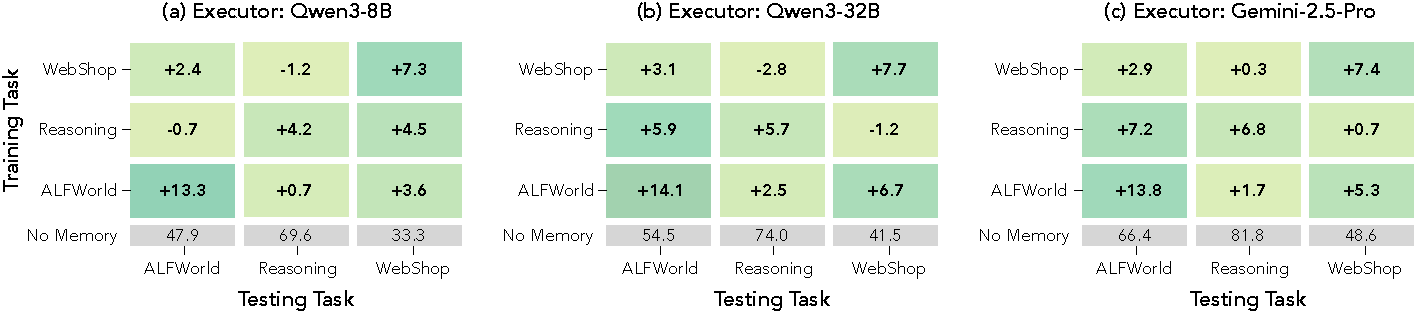
\includegraphics[width=0.95\textwidth]{figures/generalization.pdf}
\end{center}
\vspace{-3mm}
\caption{Cross-task generalization results of \ours{} with (a) Qwen3-8B, (b) Qwen3-32B, and (c) Gemini-2.5-Pro as frozen executors. We plot relative improvement with baselines from \textbf{\textcolor{lightgreen}{least}} to \textbf{\textcolor{deepgreen}{most}}.}
\label{fig: task_generalization}
\vspace{-5mm}
\end{figure}

\noindent\textbf{\ours{} is transferable and remains effective for different agent executors.}
During training, we use Qwen3-8B as the executor. To test whether \ours{} brings improvement for executors that are not seen in training, we pair the trained skill curator with different executors. As shown in Table~\ref{table: alfworld} and \ref{tab:merged_results}, \ours{} consistently improves a wide range of frozen executors across benchmarks, from open-source models (Qwen3-8B, Qwen3-32B) to frontier models (Gemini-2.5-Pro). On ALFWorld, it lifts the average success rate of Qwen3-8B from 47.9 to 61.2 and Gemini-2.5-Pro from 66.4 to 80.2, demonstrating compatibility with executors of varying capacity. Notably, using Gemini-2.5-Pro directly as the curator (\ours{}-gemini) underperforms our trained curator, especially when paired with the smaller Qwen3-8B executor. This highlights a curator-executor mismatch: stronger reasoning ability alone does not guarantee effective skill curation, as frontier-generated skills may be misaligned with the executor's capacity or usage patterns. By contrast, \ours{} learns executor-grounded curation behaviors through RL, producing skills that better match the downstream agent.

\noindent\textbf{\ours{} delivers consistent performance improvement when generalized to different task domains.} Figure~\ref{fig: task_generalization} shows that the skill curator learned by \ours{} transfers well across different tasks. While training and testing on the same task often gives the strongest gain, most off-diagonal entries still bring performance improvement over baselines, indicating that \ours{} captures reusable skills beyond task-specific heuristics. Specifically, skill curator $\pi_{s}$ learned from reasoning tasks transfer particularly well to the two agentic tasks, likely because they contain more abstract and high-level strategies, such as decomposition, verification, and adaptive planning, which are broadly useful across settings. In contrast, skills learned from WebShop or ALFWorld are more tied to environment-specific knowledge, making them less transferable across tasks.